% Copyright 2004 by Till Tantau <tantau@users.sourceforge.net>.
%
% In principle, this file can be redistributed and/or modified under
% the terms of the GNU Public License, version 2.
%
% However, this file is supposed to be a template to be modified
% for your own needs. For this reason, if you use this file as a
% template and not specifically distribute it as part of a another
% package/program, I grant the extra permission to freely copy and
% modify this file as you see fit and even to delete this copyright
% notice. 

\documentclass[xcolor=table]{beamer}
\usepackage{menukeys}[os=win]
\usepackage{textcomp}
\usepackage{tcolorbox}
\usepackage{listings}
\lstset{
  basicstyle=\tiny\ttfamily,
}

% There are many different themes available for Beamer. A comprehensive
% list with examples is given here:
% http://deic.uab.es/~iblanes/beamer_gallery/index_by_theme.html
% You can uncomment the themes below if you would like to use a different
% one:
%\usetheme{AnnArbor}
%\usetheme{Antibes}
%\usetheme{Bergen}
%\usetheme{Berkeley}
%\usetheme{Berlin}
%\usetheme{Boadilla}
%\usetheme{boxes}
%\usetheme{CambridgeUS}
%\usetheme{Copenhagen}
%\usetheme{Darmstadt}
%\usetheme{default}
%\usetheme{Frankfurt}
%\usetheme{Goettingen}
%\usetheme{Hannover}
%\usetheme{Ilmenau}
\usetheme{JuanLesPins}
%\usetheme{Luebeck}
%\usetheme{Madrid}
%\usetheme{Malmoe}
%\usetheme{Marburg}
%\usetheme{Montpellier}
%\usetheme{PaloAlto}
%\usetheme{Pittsburgh}
%\usetheme{Rochester}
%\usetheme{Singapore}
%\usetheme{Szeged}
%\usetheme{Warsaw}
\setbeamerfont{block body}{size=\small}
\title{KF5004 - \texttt{MySQL} and \texttt{PHPMyAdmin}}

% A subtitle is optional and this may be deleted
% \subtitle{(Using proximity detection)}

\author{Dr.~Neil~Eliot\inst{1} / Dr.~Alun~Moon\inst{1}}
% - Give the names in the same order as the appear in the paper.
% - Use the \inst{?} command only if the authors have different
%   affiliation.

%\renewcommand\appendixname{Appendix}

\institute[Northumbria University] % (optional, but mostly needed)
{
  \inst{1}
  Department of Computer and Information Sciences\\
  University of Northumbria
  % \and
  % \inst{2}
  % Department of Theoretical Philosophy\\
  % University of Elsewhere
}
% - Use the \inst command only if there are several affiliations.
% - Keep it simple, no one is interested in your street address.

\date{Session 10}
% - Either use conference name or its abbreviation.
% - Not really informative to the audience, more for people (including
%   yourself) who are reading the slides online

\subject{Introduction}
% This is only inserted into the PDF information catalog. Can be left
% out. 

% If you have a file called "university-logo-filename.xxx", where xxx
% is a graphic format that can be processed by latex or pdflatex,
% resp., then you can add a logo as follows:

% \pgfdeclareimage[height=0.5cm]{university-logo}{university-logo-filename}
% \logo{\pgfuseimage{university-logo}}

% Delete this, if you do not want the table of contents to pop up at
% the beginning of each subsection:
% \AtBeginSubsection[]
% {
%   \begin{frame}<beamer>{Outline}
%     \tableofcontents[currentsection,currentsubsection]
%   \end{frame}
% }

% Let's get started

\begin{document}

\begin{frame}
  \titlepage
\end{frame}

\begin{frame}{Introduction}
  \tableofcontents
  % You might wish to add the option [pausesections]
\end{frame}

% Section and subsections will appear in the presentation overview
% and table of contents.

\section{Introduction}
\subsection{Background}
\begin{frame}{What is \texttt{MySQL}?}
  \begin{itemize}
    \item \texttt{MySQL} is described as:
      \begin{itemize}
        \item An \texttt{RDBMS} (\textbf{R}elational \textbf{D}ata\textbf{B}ase \textbf{M}anagement \textbf{S}ystem)
        \item Fast
        \item Multi-threaded
        \item Multi-user
        \item Robust 
      \end{itemize}
    \item It is intended for mission-critical, heavy-load production systems as well as for embedding into mass-deployed software.
  \end{itemize}
\end{frame}

\begin{frame}{What is \texttt{MySQL}?}
  \begin{itemize}
    \item It is based on relational/set theory.
      \begin{itemize}
        \item Relational algebra ($\sigma,\pi,\theta,\bowtie$). 
      \end{itemize}
    \item It is a multi-user environment that supports multiple databases concurrently.
    \item Each database usually contains the data associated with a single application.
    \item There is a meta database used to store the structure of each database, user accounts and access rights.
  \end{itemize}
\end{frame}

\begin{frame}{What is \texttt{MySQL}?}
  \begin{figure}
    \begin{center}
      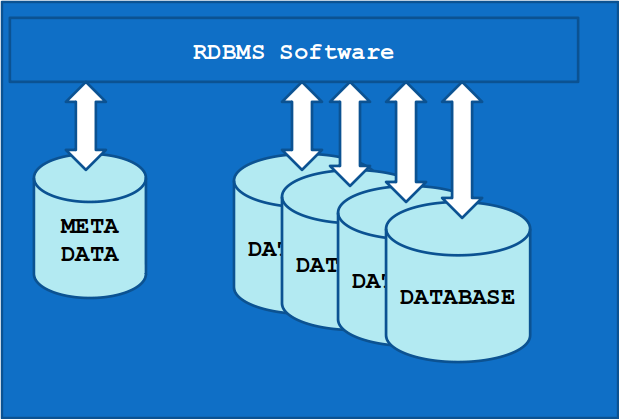
\includegraphics[width=0.8\linewidth]{What.png}
    \end{center}
  \end{figure}
\end{frame}

\begin{frame}{What is \texttt{MySQL}?}
  \begin{figure}
    \begin{center}
      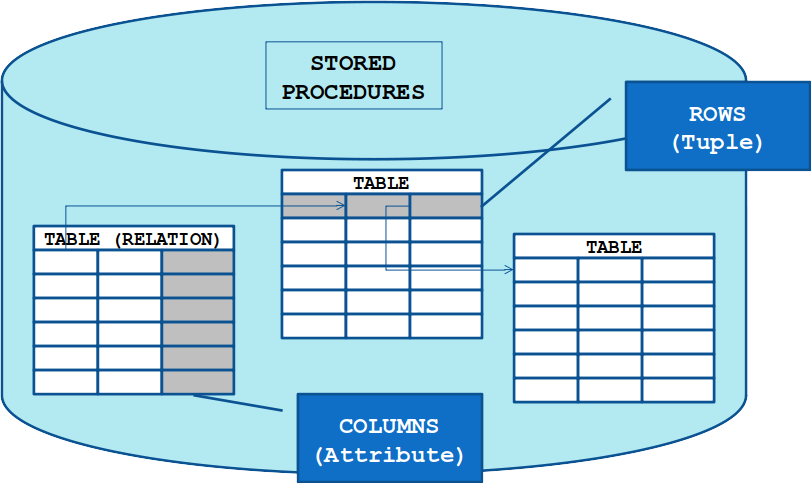
\includegraphics[width=0.8\linewidth]{What2.png}
    \end{center}
  \end{figure}
\end{frame}

\section{Installation}
\subsection{\texttt{MySQL} Server Installation}
\begin{frame}{\texttt{MySQL} Installation}
  \begin{itemize}
    \item Like most services you need to install it from the \texttt{Ubuntu Repository}.
      \begin{itemize}
        \item \texttt{\$sudo apt-get install mysql-server}
      \end{itemize}
  \end{itemize}
  \begin{tcolorbox}
    \begin{center}
      \scriptsize Default install locks access to \texttt{localhost} after installation you need to change the \texttt{BIND-ADDRESS} if you are going to use remote clients.
    \end{center}
  \end{tcolorbox}
\end{frame}

\begin{frame}[fragile]{\texttt{MySQL} Server Installation}
  \begin{tcolorbox}
    \lstset{
      basicstyle=\tiny\ttfamily,
    }
    \begin{lstlisting}
Reading package lists... Done
Building dependency tree
Reading state information... Done
The following additional packages will be installed:
  libaio1 libcgi-fast-perl libcgi-pm-perl libencode-locale-perl
  libevent-core-2.1-6 libfcgi-perl libhtml-parser-perl 
  libhtml-tagset-perl libhtml-template-perl libhttp-date-perl 
  libhttp-message-perl libio-html-perl liblwp-mediatypes-perl 
  libtimedate-perl liburi-perl mysql-client-5.7
  mysql-client-core-5.7 mysql-common mysql-server-5.7 mysql-server-core-5.7
Suggested packages:
  libdata-dump-perl libipc-sharedcache-perl libwww-perl mailx tinyca
The following NEW packages will be installed:
  libaio1 libcgi-fast-perl libcgi-pm-perl libencode-locale-perl
  libevent-core-2.1-6 libfcgi-perl libhtml-parser-perl libhtml-tagset-perl
  libhtml-template-perl libhttp-date-perl libhttp-message-perl 
  libio-html-perl liblwp-mediatypes-perl libtimedate-perl liburi-perl 
  mysql-client-5.7 mysql-client-core-5.7 mysql-common mysql-server 
  mysql-server-5.7 mysql-server-core-5.7
0 upgraded, 21 newly installed, 0 to remove and 5 not upgraded.
Need to get 21.0 MB of archives.
After this operation, 162 MB of additional disk space will be used.
Do you want to continue? [Y/n]
    \end{lstlisting}
  \end{tcolorbox}
\end{frame}

\begin{frame}[fragile]{\texttt{MySQL} Server Installation}
  \begin{itemize}
    \item A security package can be added to improve the robustness of \texttt{MySQL}.
    \begin{itemize}
      \item \texttt{\$sudo mysql\_secure\_installation}
    \end{itemize}
  \end{itemize}
  \begin{tcolorbox}
    \lstset{
      basicstyle=\tiny\ttfamily,
    }
    \begin{lstlisting}
Securing the MySQL server deployment.
    
Connecting to MySQL using a blank password.
      
VALIDATE PASSWORD PLUGIN can be used to test passwords
and improve security. It checks the strength of password
and allows the users to set only those passwords which are
secure enough. Would you like to setup VALIDATE PASSWORD plugin?
      
Press y|Y for Yes, any other key for No:
    \end{lstlisting}
  \end{tcolorbox}
Continued...
\end{frame}

\begin{frame}[fragile]{\texttt{MySQL} Server Installation}
  \begin{itemize}
    \item A security package can be added to improve the robustness of \texttt{MySQL}.
    \begin{itemize}
      \item \texttt{\$sudo mysql\_secure\_installation}
    \end{itemize}
  \end{itemize}
  \begin{tcolorbox}
    \lstset{
      basicstyle=\tiny\ttfamily,
    }
    \begin{lstlisting}
Press y|Y for Yes, any other key for No: Y

There are three levels of password validation policy:
      
LOW    Length >= 8
MEDIUM Length >= 8, numeric, mixed case, and special …
STRONG Length >= 8, numeric, mixed case, special characters …
Please enter 0 = LOW, 1 = MEDIUM and 2 = STRONG: 0
    \end{lstlisting}
  \end{tcolorbox}
  \begin{tcolorbox}
    To make things a bit easier in the module select \texttt{0} for \texttt{LOW} and set the password to \texttt{northumbria}
  \end{tcolorbox}
\end{frame}

\section{Post installation}
\subsection{Security}
\begin{frame}{Access to the \texttt{MySQL} Server}
  \begin{itemize}
    \item Access to \texttt{MySQL} server can be limited to specific network.
      \begin{itemize}
        \item \texttt{/etc/mysql/mysql.conf.d/mysqld.cnf}
      \end{itemize}
    \item Specifying a specific \texttt{IP} Address binds \texttt{MySQL} to that network card.
      \begin{itemize}
        \item \texttt{bind-address=192.168.101.5}
        \item Useful when the machine is attached to more than one network.
      \end{itemize}
    \item Specifying a \texttt{NULL} (\texttt{0.0.0.0}) address allows open access to the server.
    \item Specifying \texttt{127.0.0.1} limits access to \texttt{localhost} only.
      \begin{itemize}
        \item Often used on single server intranet implementations.
      \end{itemize}
  \end{itemize}
\end{frame}

\subsection{Security}
\begin{frame}{Quick recap - Where does \texttt{MySQL} fit in?}
  \begin{figure}
    \begin{center}
      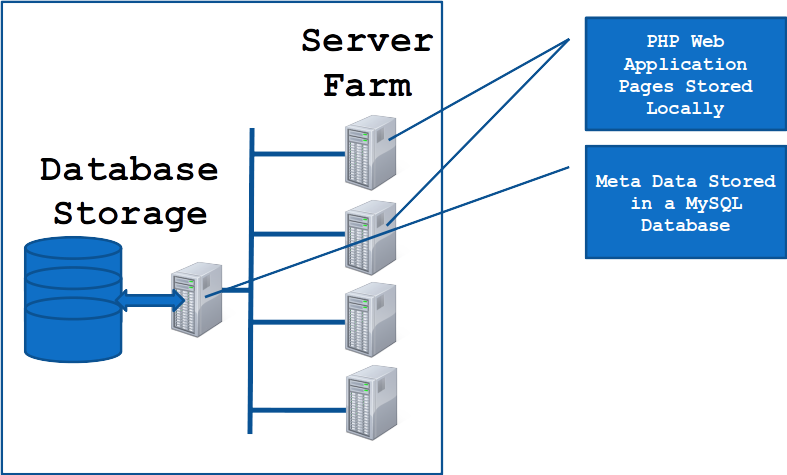
\includegraphics[width=0.8\linewidth]{MySQLWhere.png}
    \end{center}
  \end{figure}
\end{frame}

\subsection{Client Connectivity}
\begin{frame}[fragile]{Install \texttt{MySQL} Client software}
  \begin{itemize}
    \item Access to a \texttt{MySQL} server requires specific libraries and utilities.
    \item As with most software it is installed from the repositories.
      \begin{itemize}
        \item \texttt{\$sudo apt-get install mysql-client}
      \end{itemize}
  \end{itemize}
  \begin{tcolorbox}
    \lstset{
      basicstyle=\tiny\ttfamily,
    }
    \begin{lstlisting}
Reading package lists... Done
Building dependency tree
Reading state information... Done
The following NEW packages will be installed:
  mysql-client
0 upgraded, 1 newly installed, 0 to remove and 31 not upgraded.
Need to get 6,174 B of archives.
After this operation, 98.3 kB of additional disk space will be used.
Get:1 http://us.archive.ubuntu.com/ubuntu/ oneiric/main mysql-client 
  all 5.1.58-1ubuntu1 [6,174 B]
Fetched 6,174 B in 0s (30.0 kB/s)
Selecting previously deselected package mysql-client.
...
    \end{lstlisting}
  \end{tcolorbox}
\end{frame}

\begin{frame}{\texttt{PHP} and \texttt{MySQL}}
  \begin{figure}
    \begin{center}
      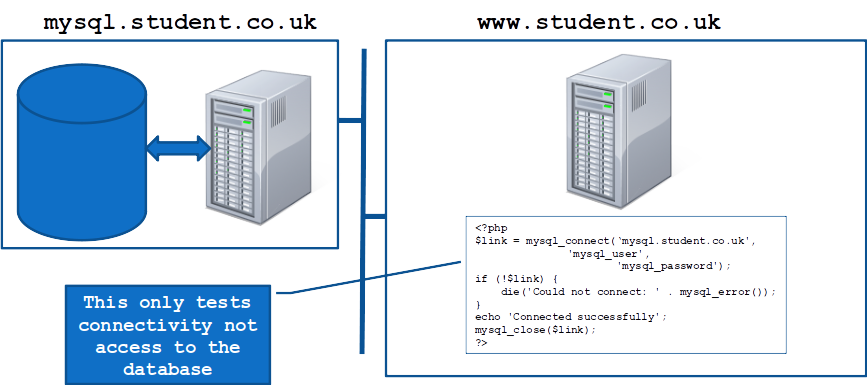
\includegraphics[width=1\linewidth]{Connectivity.png}
    \end{center}
  \end{figure}
\end{frame}

\begin{frame}[fragile]{\texttt{PHP} to \texttt{MySQL} test script}
  \begin{tcolorbox}
    \lstset{
      basicstyle=\tiny\ttfamily,
    }
    \begin{lstlisting}
      <?php
      $link = mysql_connect('mysql.student.co.uk',
               'mysql_user','mysql_password');
      if (!$link) {
        die('Could not connect:' . mysql_error());
      }
      echo 'Connected successfully';
      mysql_close($link);
      ?>
    \end{lstlisting}
  \end{tcolorbox}
  \begin{tcolorbox}
    \small\texttt{https://php.net/manual/en/function.mysql-connect.php}
  \end{tcolorbox}
\end{frame}

\subsection{Managing \texttt{MySQL}}
\begin{frame}{What is \texttt{SQL}?}
  \begin{itemize}
    \item \texttt{MySQL} is an application that runs in the background (\texttt{daemon}) and you interact with it via \texttt{SQL} commands.
    \item There are several different types of commands.
      \begin{itemize}
        \item \texttt{DDL}
        \item \texttt{DML}
        \item \texttt{TCL}
        \item \texttt{DCL}
      \end{itemize}
  \end{itemize}
\end{frame}

\begin{frame}{What is \texttt{SQL}?}
  \begin{itemize}
    \item Data Definition Language (\texttt{DDL})
      \begin{itemize}
        \item These \texttt{SQL} commands are used for creating, modifying, and dropping the structure of database objects. The commands are \texttt{CREATE, ALTER, DROP, RENAME,} and \texttt{TRUNCATE}.
      \end{itemize}
    \item Data Manipulation Language (\texttt{DML})
      \begin{itemize}
        \item These \texttt{SQL} commands are used for storing, retrieving, modifying, and deleting data. These commands are \texttt{SELECT, INSERT, UPDATE,} and \texttt{DELETE}.
      \end{itemize}
    \item Transaction Control Language (\texttt{TCL})
      \begin{itemize}
        \item These \texttt{SQL} commands are used for managing changes affecting the data. These commands are \texttt{COMMIT, ROLLBACK,} and \texttt{SAVEPOINT}.
      \end{itemize}
    \item Data Control Language (\texttt{DCL})
      \begin{itemize}
        \item These \texttt{SQL} commands are used for providing security to database objects. These commands are \texttt{GRANT} and \texttt{REVOKE}.
      \end{itemize}
  \end{itemize}
\end{frame}

\begin{frame}{Create Users}
  \begin{itemize}
    \item \texttt{MySQL} is a multi-user system so you also need to be able to manage users of the system.
    \item The \texttt{CREATE} command adds users to be added.
    \item Data Manipulation Language (\texttt{DML})
      \begin{itemize}
        \item \texttt{CREATE USER \textit{user\_specification}}
        \item \texttt{\textit{user\_specification:} [IDENTIFIED BY [PASSWORD] 'password']} 
      \end{itemize}
  \end{itemize}
\end{frame}

\begin{frame}{Create Users}
  \begin{itemize}
    \item The \texttt{CREATE USER} statement creates new \texttt{MySQL} account. 
    \item To use the command you must have the global \texttt{CREATE USER} privilege or the\texttt{INSERT} privilege for the \texttt{mysql} database. 
    \item For each account; \texttt{CREATE USER} creates a new row in the \texttt{mysql.user table} and assigns the account no privileges. 
    \begin{itemize}
      \item An error occurs if the account already exists.
    \end{itemize}
  \end{itemize}
  \begin{tcolorbox}
    \small\texttt{CREATE USER 'webaccount' IDENTIFIED BY 'password';}
  \end{tcolorbox}
\end{frame}

\begin{frame}{Managing \texttt{MySQL}}
  \begin{itemize}
    \item There are several management interfaces.
    \begin{itemize}
      \item \texttt{CLI} - The command line interface (\texttt{mysql}) provides an environment that allows \texttt{SQL} commands to be entered for all management operations.
      \item \texttt{Graphical Interface} - \texttt{MySQL Workbench} provides \texttt{DBA}s and developers an integrated tools environment for:  
        \begin{itemize}
          \item Database Design and Modelling
          \item \texttt{SQL} Development
          \item Database Administration
          \item Database Migration
        \end{itemize}
      \item \texttt{Web Interface} - \texttt{PHPMyAdmin} is a web tool that can be installed on a web server (usually the same server as the database) to provide an \texttt{HTML} based interface to the Database.
    \end{itemize}
  \end{itemize}
  \begin{tcolorbox}
    \begin{center}
      \small This module covers some of \texttt{CLI} and \texttt{PHPMyAdmin}      
    \end{center}
  \end{tcolorbox}
\end{frame}

\begin{frame}{Managing \texttt{MySQL} - \texttt{CLI}}
  \begin{itemize}
    \item Connecting to the \texttt{MySQL} Server:
      \begin{itemize}
        \item \texttt{\$sudo mysql -u root}    
      \end{itemize}
    \item Show all the databases:
      \begin{itemize}
        \item \texttt{mysql> show databases;}    
      \end{itemize}
    \item Select a database:
      \begin{itemize}
        \item \texttt{mysql> use <database name>;}
        \item e.g. \texttt{use intranet;}    
      \end{itemize}
    \item List the tables in a database:
      \begin{itemize}
        \item \texttt{mysql> show tables;}
      \end{itemize}
    \item Show the structure of a table: 
      \begin{itemize}
        \item \texttt{mysql> desc <tablename>;}
        \item e.g. \texttt{show users;}    
      \end{itemize}
  \end{itemize}
\end{frame}

\begin{frame}{Managing \texttt{MySQL} - \texttt{CLI}}
  \begin{itemize}
    \item One of the system databases in a \texttt{MySQL} database is the \texttt{mysql} database.
    \item It contains all the metadata required to manage users, access rights, and security for the system.
    \item Two of those metadata tables are:-
      \begin{itemize}
        \item \texttt{user} - Contains the data about users and their system security rights.
        \item \texttt{db} - Contains the database names, authorised users and their level of access.
      \end{itemize}
  \end{itemize}
\end{frame}

\begin{frame}{Managing \texttt{MySQL} - \texttt{CLI}}
  \begin{itemize}
    \item Creating Users and Databases.
      \begin{itemize}
        \item You must be logged in with an account that has full rights to the server.
          \begin{itemize}
            \item After installation their will be only one account with these privileges - \texttt{root}
          \end{itemize}
        \item To create a user.
          \begin{itemize}
            \item \texttt{mysql> CREATE USER 'webaccount'@'\%' IDENTIFIED BY 'Northumbria2018!';}
          \end{itemize}
        \item To create a database.
          \begin{itemize}
            \item \texttt{mysql> CREATE DATABASE webDB;}
          \end{itemize}
      \end{itemize}
  \end{itemize}
\end{frame}

\begin{frame}{Managing \texttt{MySQL} - \texttt{CLI}}
  \begin{itemize}
    \item Creating Users and Databases.
      \begin{itemize}
        \item Although you now have a \texttt{user} and a \texttt{database} the user has no rights to use the database.
          \begin{itemize}
            \item The GRANT command allows rights to added to a user.
            \item The REVOKE command allows rights to be removed.
          \end{itemize}
        \item To add full control of a \texttt{database} to a \texttt{user} you grant \texttt{ALL} privileges.
          \begin{itemize}
            \item \texttt{mysql> GRANT ALL ON webDB to 'webaccount'@'\%';}
          \end{itemize}
      \end{itemize}
  \end{itemize}
\end{frame}

\begin{frame}[fragile]{Managing \texttt{MySQL} - \texttt{CLI}}
  \begin{tcolorbox}
    \lstset{
      basicstyle=\tiny\ttfamily,
    }
    \begin{lstlisting}
student@a123456789:~$ sudo mysql -u root
...
mysql> create user 'webaccount'@'%' identified by 'Northumbria2018!';
Query OK, 0 rows affected (0.01 sec)

mysql> create database webdb;
Query OK, 1 row affected (0.14 sec)

mysql> grant all on webdb.* to webaccount;
Query OK, 0 rows affected (0.01 sec)

mysql> flush privileges;
Query OK, 0 rows affected (0.00 sec)

mysql>
    \end{lstlisting}
  \end{tcolorbox}
\end{frame}

\begin{frame}[fragile]{Managing \texttt{MySQL} - \texttt{CLI}}
  \begin{tcolorbox}
    \lstset{
      basicstyle=\Tiny\ttfamily,
    }
    \begin{lstlisting}
mysql> use mysql;
Reading table information for completion of table and column names
You can turn off this feature to get a quicker startup with -A
    
Database changed
      
mysql> select user,host,authentication_string from user;
+------------------+-----------+-------------------------------------------+
| user             | host      | authentication_string                     |
+------------------+-----------+-------------------------------------------+
| root             | localhost |                                           |
| mysql.session    | localhost | *THISISNOTAVALIDPASSWORDTHATCANBEUSEDHERE |
| mysql.sys        | localhost | *THISISNOTAVALIDPASSWORDTHATCANBEUSEDHERE |
| debian-sys-maint | localhost | *B833B99BDFE06465AEF2EC2F25AEE6F2009F835D |
| phpmyadmin       | localhost | *2B9F99F52869AB9C16208A88958B98285B223846 |
| admin            | %         | *2B9F99F52869AB9C16208A88958B98285B223846 |
| webaccount       | %         | *2B9F99F52869AB9C16208A88958B98285B223846 |
+------------------+-----------+-------------------------------------------+
7 rows in set (0.00 sec)
     
mysql>     
    \end{lstlisting}
  \end{tcolorbox}
\end{frame}

\begin{frame}[fragile]{Managing \texttt{MySQL} - \texttt{CLI}}
  \begin{tcolorbox}
    \lstset{
      basicstyle=\Tiny\ttfamily,
    }
    \begin{lstlisting}
mysql> select host,db,user,select_priv,insert_priv,update_priv from db;
+------+-------+------------+-------------+-------------+-------------+
| host | db    | user       | select_priv | insert_priv | update_priv |
+------+-------+------------+-------------+-------------+-------------+
| %    | webdb | webaccount | Y           | Y           | Y           |
+------+-------+------------+-------------+-------------+-------------+
1 row in set (0.01 sec)
      
mysql>     
    \end{lstlisting}
  \end{tcolorbox}
\end{frame}

\begin{frame}[fragile]{Managing \texttt{MySQL} - \texttt{CLI}}
  \begin{tcolorbox}
    \lstset{
      basicstyle=\Tiny\ttfamily,
    }
    \begin{lstlisting}
student@a123456789:~$ mysql -u webaccount -p
Enter password:
Welcome to the MySQL monitor.  Commands end with ; or \g.
Your MySQL connection id is 70
Server version: 5.7.22-0ubuntu18.04.1 (Ubuntu)
      
Copyright (c) 2000, 2018, Oracle and/or its affiliates. All rights reserved.
     
Oracle is a registered trademark of Oracle Corporation and/or its
affiliates. Other names may be trademarks of their respective
owners.
      
Type 'help;' or '\h' for help. Type '\c' to clear the current input statement.
      
mysql> show databases;
+--------------------+
| Database           |
+--------------------+
| information_schema |
| webaccount         |
+--------------------+
2 rows in set (0.00 sec)
      
mysql>
    \end{lstlisting}
  \end{tcolorbox}
\end{frame}

\begin{frame}{Managing \texttt{MySQL} - \texttt{PHPMyAdmin}}
  \begin{itemize}
    \item Managing \texttt{MySQL} via the \texttt{CLI} can be complicated and requires a lot of commands to be memorised. 
    \item \texttt{MySQL} can also be managed via the popular \texttt{PHPMyAdmin} web interface.
    \item Most \texttt{Unix} variants now supply this as a package that can be directly installed.
    \item On most platforms \texttt{Apache} is classed as a dependency and is automatically installed when \texttt{PHPMyAdmin} is install via a package manager. Some require either \texttt{lightpd} or \texttt{Apache} to be pre-installed.
  \end{itemize}
\end{frame}

\begin{frame}{Managing \texttt{MySQL} - \texttt{PHPMyAdmin}}
  \begin{itemize}
    \item \texttt{PHPMyAdmin} is install on Ubuntu Server using the command:
      \begin{itemize}
        \item \texttt{\$sudo apt-get install phpmyadmin}
      \end{itemize}
  \end{itemize}
\end{frame}

\begin{frame}[fragile]{Managing \texttt{MySQL} - \texttt{PHPMyAdmin}}
  \begin{tcolorbox}
    \lstset{
      basicstyle=\Tiny\ttfamily,
    }
    \begin{lstlisting}
student@a123456789:~$ sudo apt-get install phpmyadmin
[sudo] password for student:
Reading package lists... Done
Building dependency tree
Reading state information... Done
The following additional packages will be installed:
  dbconfig-common dbconfig-mysql fontconfig-config fonts-dejavu-core
  javascript-common libfontconfig1 libgd3 libjbig0 libjpeg-turbo8 libjpeg8
  libjs-jquery libjs-sphinxdoc libjs-underscore libtiff5 libwebp6 libxpm4
  libzip4 php-bz2 php-curl php-gd php-mbstring php-pear php-php-gettext
  php-phpseclib php-tcpdf php-xml php-zip php7.2-bz2 php7.2-curl php7.2-gd
  php7.2-mbstring php7.2-xml php7.2-zip
Suggested packages:
  libgd-tools php-libsodium php-mcrypt php-gmp php-imagick www-browser
The following NEW packages will be installed:
  dbconfig-common dbconfig-mysql fontconfig-config fonts-dejavu-core
  javascript-common libfontconfig1 libgd3 libjbig0 libjpeg-turbo8 libjpeg8
  libjs-jquery libjs-sphinxdoc libjs-underscore libtiff5 libwebp6 libxpm4
  libzip4 php-bz2 php-curl php-gd php-mbstring php-pear php-php-gettext
  php-phpseclib php-tcpdf php-xml php-zip php7.2-bz2 php7.2-curl php7.2-gd
  php7.2-mbstring php7.2-xml php7.2-zip phpmyadmin
0 upgraded, 34 newly installed, 0 to remove and 5 not upgraded.
Need to get 15.6 MB of archives.
After this operation, 60.1 MB of additional disk space will be used.
Do you want to continue? [Y/n]
    \end{lstlisting}
  \end{tcolorbox}
\end{frame}

\begin{frame}{Managing \texttt{MySQL} - \texttt{PHPMyAdmin}}
  \begin{figure}
    \begin{center}
      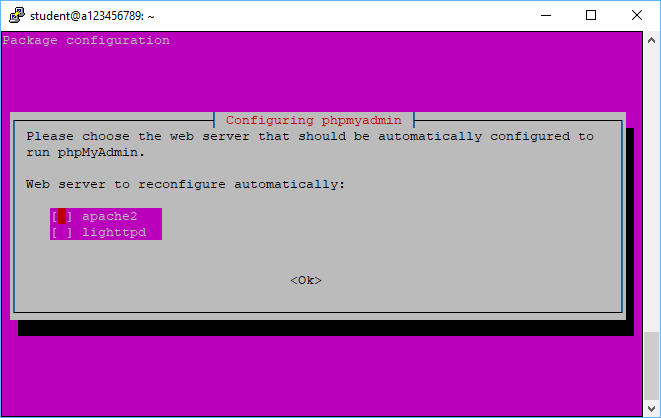
\includegraphics[width=1\linewidth]{MySQLInstall1.png}
    \end{center}
  \end{figure}
\end{frame}

\begin{frame}{Managing \texttt{MySQL} - \texttt{PHPMyAdmin}}
  \begin{figure}
    \begin{center}
      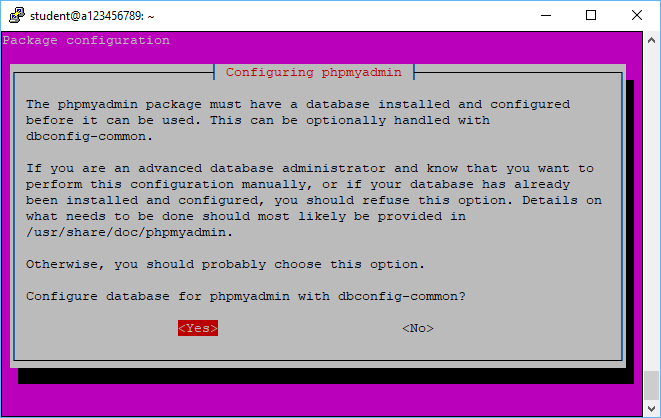
\includegraphics[width=1\linewidth]{MySQLInstall2.png}
    \end{center}
  \end{figure}
\end{frame}

\begin{frame}{Managing \texttt{MySQL} - \texttt{PHPMyAdmin}}
  \begin{figure}
    \begin{center}
      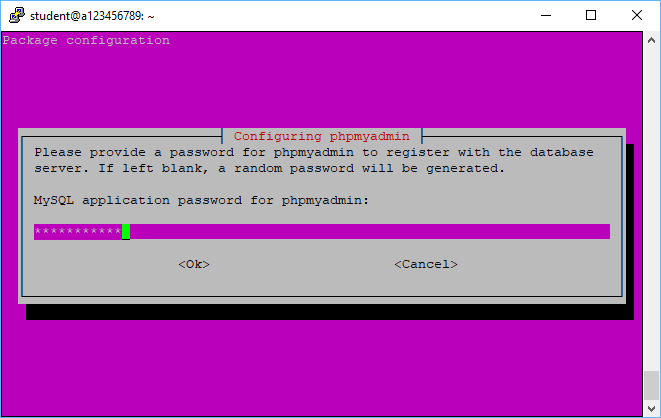
\includegraphics[width=1\linewidth]{MySQLInstall3.png}
    \end{center}
  \end{figure}
\end{frame}

\begin{frame}{Managing \texttt{MySQL} - \texttt{PHPMyAdmin}}
  \begin{figure}
    \begin{center}
      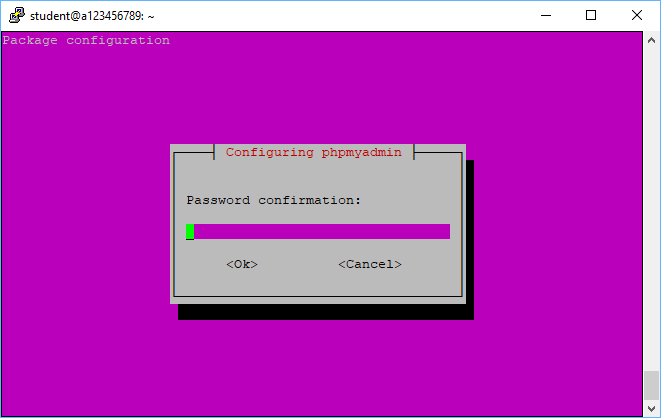
\includegraphics[width=1\linewidth]{MySQLInstall4.png}
    \end{center}
  \end{figure}
\end{frame}

\begin{frame}{\texttt{PHPMyAdmin} - Post Install}
  \begin{itemize}
    \item When \texttt{MySQL} is secured the \texttt{MySQL root} account can only login when ran as the \texttt{Linux root} account (\texttt{sudo}).
      \begin{itemize}
        \item \textbf{PROBLEM:} You cannot use the \texttt{root} acccount through the web interface!
      \end{itemize}
    \item \textbf{SOLUTION:} To manage \texttt{MySQL} through the web interface a database account must be created with full access to the \texttt{RDBMS}.
      \begin{itemize}
        \item \texttt{CREATE USER 'admin'@'\%' IDENTIFIED BY 'Northumbria2018!';}
        \item \texttt{GRANT ALL PRIVILEGES ON *.* TO 'admin'@'\%' WITH GRANT OPTION;}
      \end{itemize}
  \end{itemize}
\end{frame}

\begin{frame}{Managing \texttt{MySQL} - \texttt{PHPMyAdmin}}
  \begin{figure}
    \begin{center}
      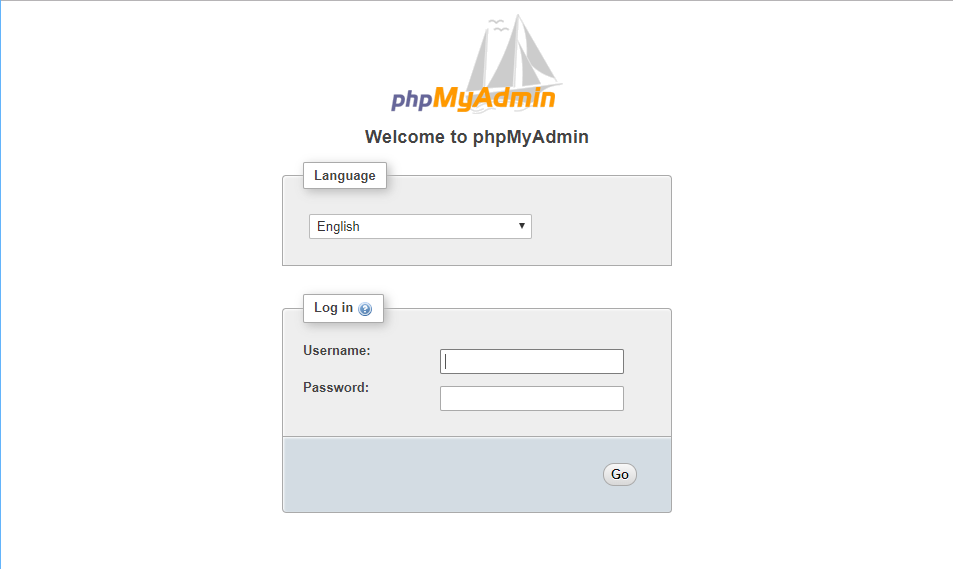
\includegraphics[width=1\linewidth]{PHPLogin.png}
    \end{center}
  \end{figure}
\end{frame}

\begin{frame}{Managing \texttt{MySQL} - \texttt{PHPMyAdmin}}
  \begin{figure}
    \begin{center}
      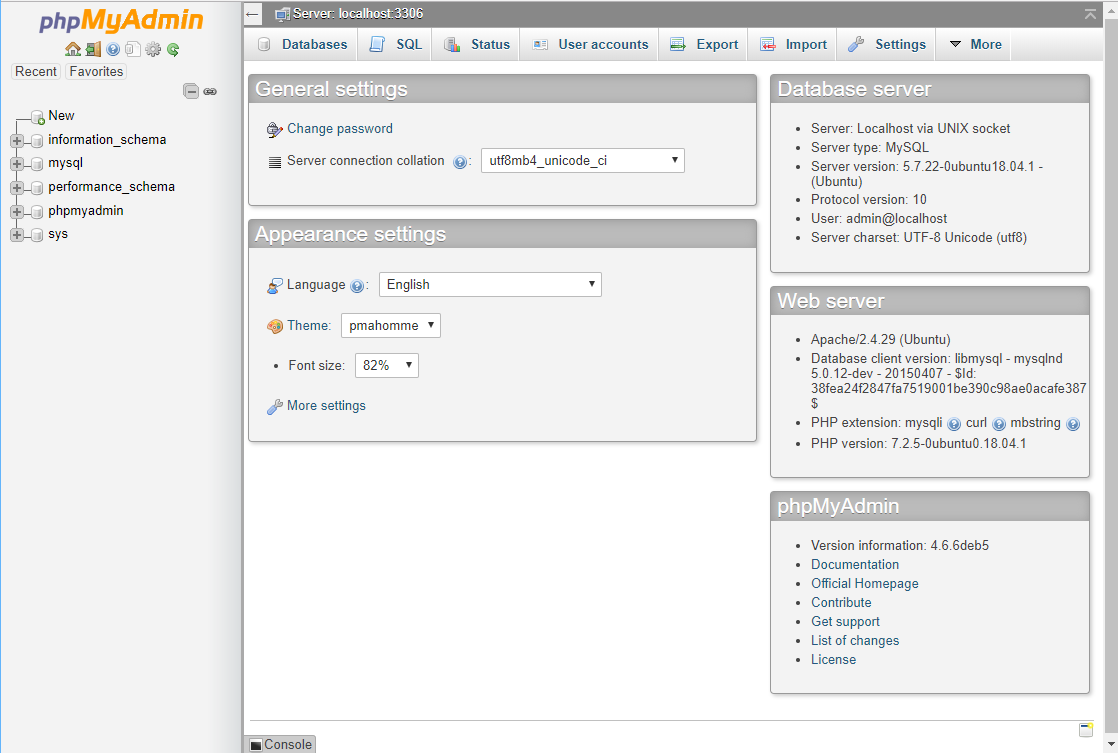
\includegraphics[width=0.9\linewidth]{PHPMyAdmin.png}
    \end{center}
  \end{figure}
\end{frame}

\begin{frame}{Managing \texttt{MySQL} - \texttt{PHPMyAdmin}}
  \begin{figure}
    \begin{center}
      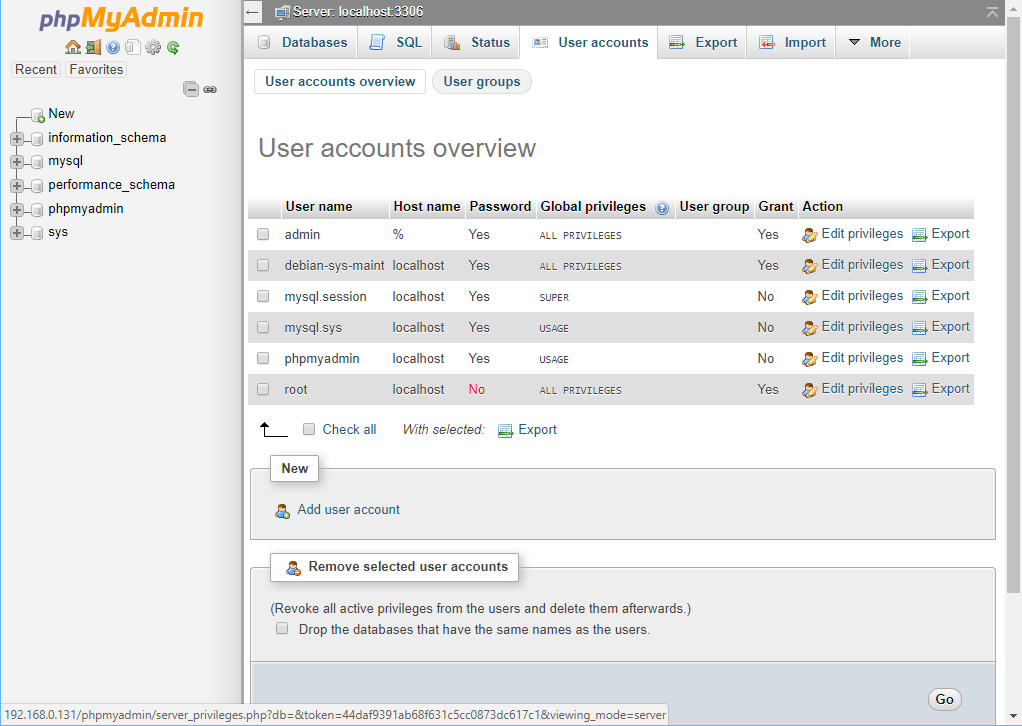
\includegraphics[width=0.9\linewidth]{Accounts.png}
    \end{center}
  \end{figure}
\end{frame}

\begin{frame}{Managing \texttt{MySQL} - \texttt{PHPMyAdmin}}
  \begin{figure}
    \begin{center}
      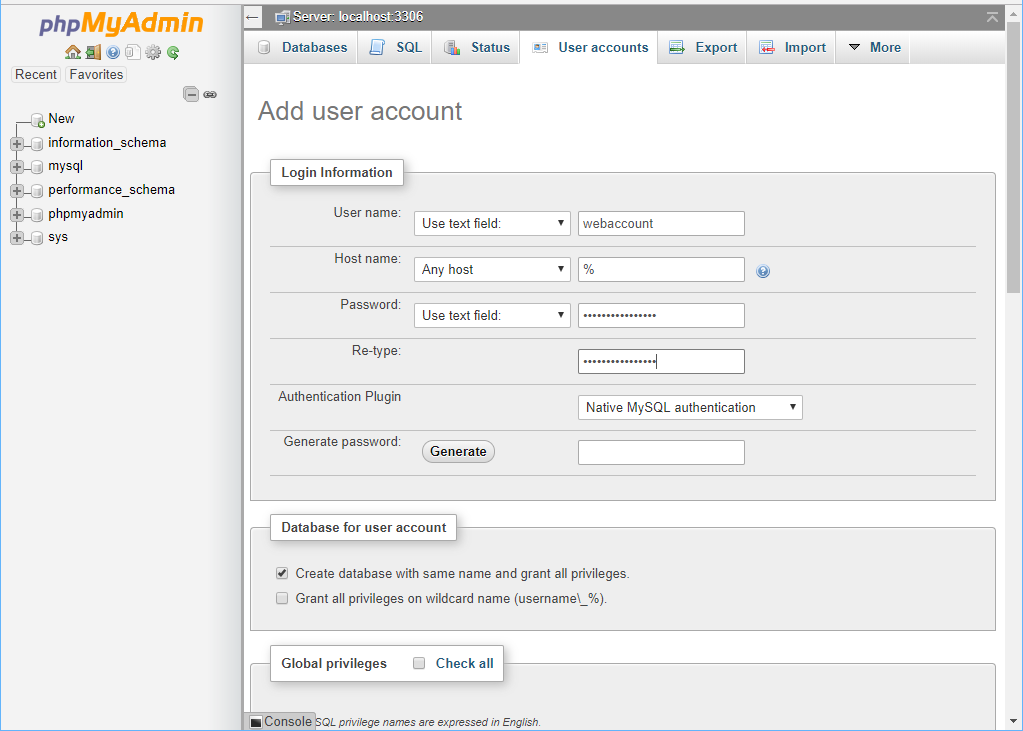
\includegraphics[width=0.9\linewidth]{Accounts2.png}
    \end{center}
  \end{figure}
\end{frame}

\begin{frame}{Managing \texttt{MySQL} - \texttt{PHPMyAdmin}}
  \begin{figure}
    \begin{center}
      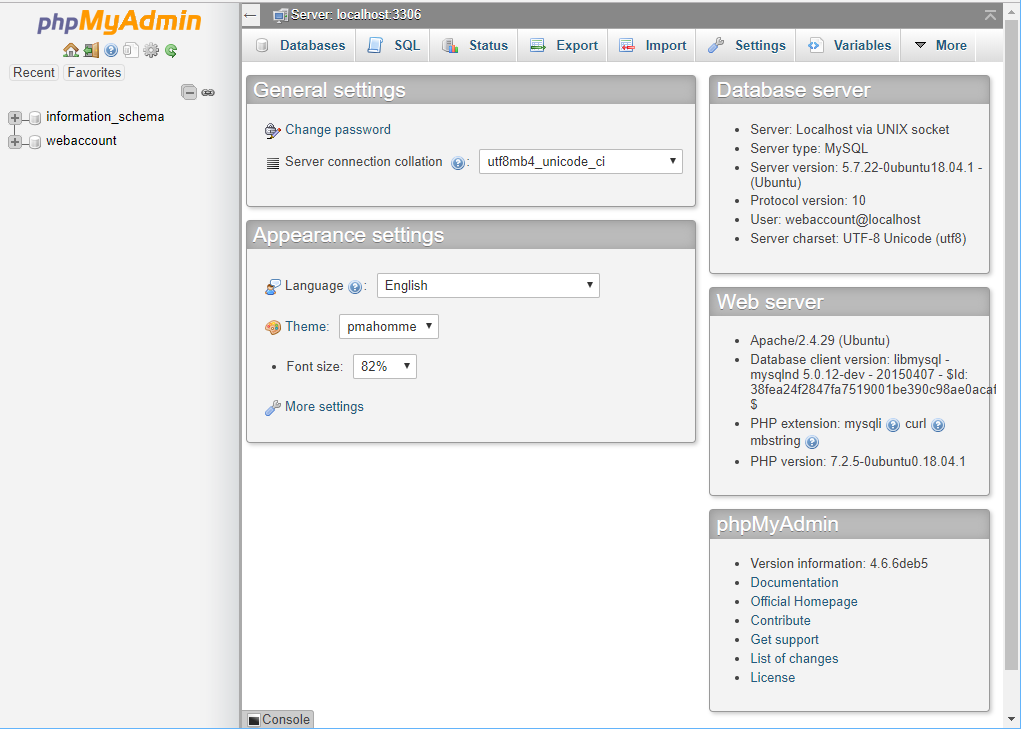
\includegraphics[width=0.9\linewidth]{Accounts3.png}
    \end{center}
  \end{figure}
\end{frame}

\begin{frame}{Managing \texttt{MySQL} - \texttt{PHPMyAdmin}}
  \begin{itemize}
    \item \texttt{PHPMyAdmin} is heavily documented.
    \begin{itemize}
      \item \texttt{http://www.phpmyadmin.net}
    \end{itemize}
  \end{itemize}
  \begin{figure}
    \begin{center}
      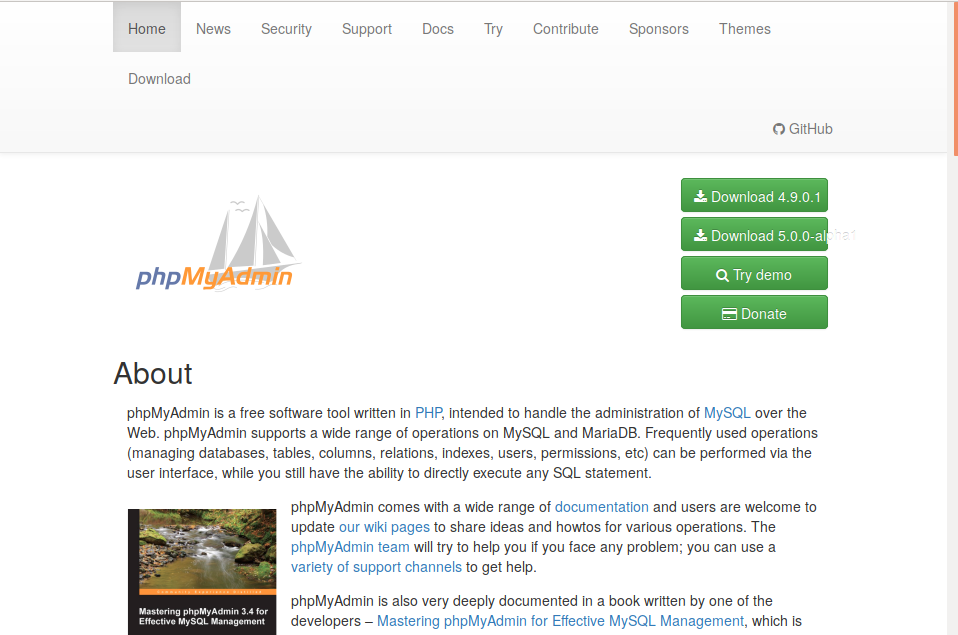
\includegraphics[width=0.7\linewidth]{PHPMyAdminSite.png}
    \end{center}
  \end{figure}
\end{frame}

\section{Advanced Deployments}
\subsection{High Availability}
\begin{frame}{\texttt{MySQL} Deployment Architectures \small{(Beyond this module)}}
  \begin{figure}
    \begin{center}
      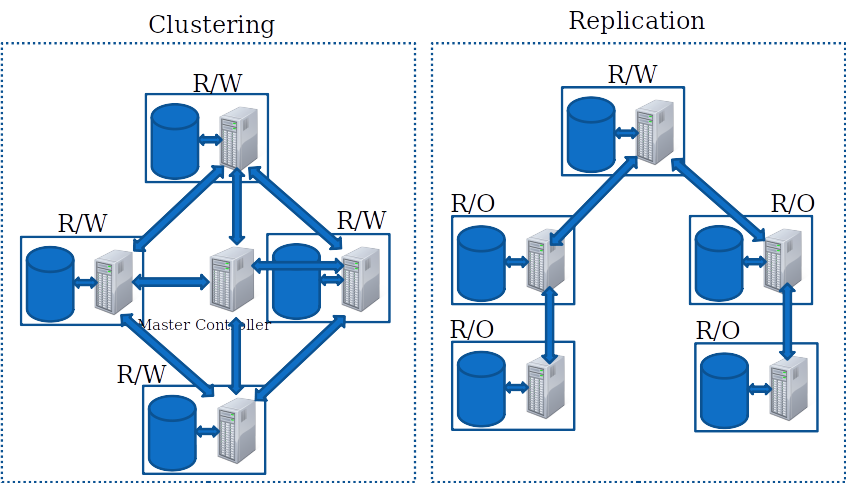
\includegraphics[width=1\linewidth]{Advanced.png}
    \end{center}
  \end{figure}
\end{frame}

\section*{Conclusion}
\begin{frame}{Conclusion}
  \begin{itemize}
    \item What is \texttt{MySQL}
    \item Where does it fit into the Web Architecture?
    \item How is it installed?
    \item How is it managed?
    \item Some Advanced Deployment option \Tiny{(Beyond the scope of the module)}
  \end{itemize}
\end{frame}

\end{document}


